\chapter{Results}
\label{chap:results}

In this chapter we will present our results from analyzing the data in the blockchain using the methods described in \cref{chap:metodology}. 
Bitcoin has a testnet used for development and testing of experimental functionality, which the LN have been tested on for longer than it has been used on the mainnet. We have used both the testnet and the mainnet in the project; our reasoning for this is the LN on the testnet is larger, and people are testing a wide array of use cases and functionality, using testnet coins without any value; on the mainnet users have Bitcoin with value, perhaps resulting in more realistic user behaviour which could impacts the data generated.
By using both Bitcoin networks we will have both edge cases and cases accurately reflecting normal user behaviour.
The testnet has its own blockchain which is publicly available in the same manner as the mainnet blockchian. Collecting data from the LN as discussed in \cref{sec:ln_analysis} was done in two intervals of one week each.
Creating a snapshot of the LN state on each block for a week results in around 1000 blocks worth of data. This should be sufficient to verify our methods of identifying relevant LN transactions, and doing this twice allowed us to make adjustments after the results of the first interval. 

\section{Method verification with LN data}

Comparing data from the LN with our data from the blockchain, provided us with results about the extent our identification methods is able to identify LN channels on the blockchain. There was three sets of data was used in these comparisons: 
\begin{itemize}
    \item The set \( \alpha \) , containing channels from the LN closed during the capture interval. 
    \item The set \( \beta \), containing channels from the blockchain identified using timelocked redeem scripts,
    \item The set  \( \gamma \), containing potential channels identified on the blockchain using 2of2 multisig scripts.
\end{itemize}

As we stated previously a LN channel uses the P2WSH 2of2 multisig type for the on chain founding - closing output - input pair. In \cref{detection_ms} we discussed how this could be used to give us a set of potential transactions being related to LN channels. Because the on-chain channel transactions must be of this type the \( \gamma \) set is guaranteed to include all channels closed in the block interval used for the search. It also means that the two other sets will be subset of \( \gamma \). So the relations between the sets should be as follows:

\begin{equation} \label{eq:1}
      \alpha \subseteq \gamma, \hspace{10pt} \beta \subseteq \gamma, \hspace{10pt} \beta \subseteq \alpha  
\end{equation}

The two first relations is explained above and is always true for the systems in its current case. The last relation however, will not hold with our data, but ideally it should be true. For this to be the case our method with timelocked redeem scripts for identifying channels should not have any false positives-i.e., identify channels which is unrelated to the LN. Additionally we should also be able to discover all closed channels in our interaction with the LN during the interval, meaning we would get the complete set of channels-i.e., \( \gamma \) contain all LN channels closed in the interval. While the timelocked scripts are very unique and therefore good for identifying channels, and theoretically one could get all LN channels by connection to the LN, this would only be true in a ideal world scenario. So as we will see with our data \( \beta \not\subseteq \alpha \), but keeping the relation in mind will be useful when analyzing the data.

\subsection{First Interval}

\begin{figure}[ht]
    \centering
    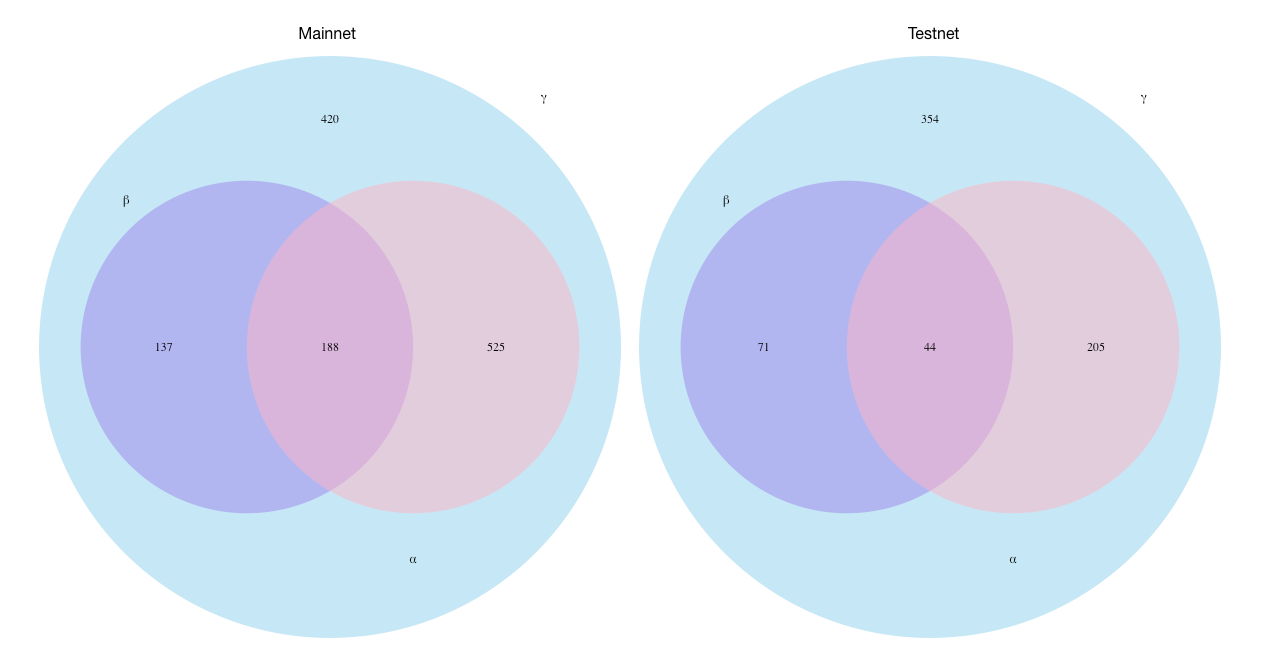
\includegraphics[width=16cm]{figures/graphs/venn_full1.png}
    \caption{Venn diagram of channel sets in interval one}
    \label{fig:venn_run1}
\end{figure}

The first collection interval on the mainnet had a length of 1151 blocks, found between block 517855 and 519005. Our modified LND implementation described in \cref{sec:ln_analysis} collected data from the LN and produced the set $\alpha$ containing 715 channels which were closed during this interval. The same interval on the blockchain was parsed two times, once identifying channels using timelocked redeem scripts, and a second time getting all potential channels using multisig identification. This resulted in a $\beta$ set containing 328 channels and a $\gamma$ set with 1271 channels shown on the left in \cref{fig:venn_run1} as a venn diagram. We can see how both $\beta$ and $\alpha$ is a subset of $\gamma$, but $\beta \not\subseteq \alpha$. The intersection $\beta \cap \alpha$ is the number of channels we identified using the timelocked redeem script which where also found trough the LN node. On the mainnet this intersection was 190 which is 36\% of the total channels in $\alpha$. This is reasonable, as the method will only discover a channel if it has been unilaterally closed as we explained in \cref{sec:bc_analysis}, and not if a channel is closed cooperatively which likely will happen more frequently. Taking the ideal world scenario $\beta \subseteq \alpha$ discussed above, into account for this data, we have a large $\beta \backslash{} \alpha$ relative compliment of $\alpha$ in $\beta$ of 138, which is 42\% of the channels in $\beta$. Having a false positive this high is very unlikely because the uniqueness of the timelocked redeem scripts, so we made the assumption that these are actually LN channels which we have not been able to capture in our interaction with the LN. The reason we made this assumption was that it is more likely that not every channel is propagated successfully to our single LN node, than there being instances of timelocked redeem scripts unrelated to the LN on the blockchain. Addiontally, as we explained in \cref{sec:ln_analysis} at least every node running the LND implementation will prune their LN graph of "zombie" channels regularly, so these will eventually no longer be propagated trough the network. This means even if our node does not prune its graph of the network, the channel will never be received in the first place. These are the likely causes of our timelocked channels not being found in the LN channel set.
Taking this into account and assuming the union $\alpha \cup \beta$ are all LN channels, the total number of LN channels closed in this interval would be 853. This would entail that 67\% of 2of2 multisig transactions in our interval is lightning channels. 
\\

For the testnet our LND node collected 838 snapshots starting on block 1290011 and ending on block 1289174. The results are very similar to the mainnet, with the intersection $\beta \cap \alpha$ being 27\% of $\alpah$,
and the $\beta \backslash{} \alpha$ relative compliment of $\alpha$ in $\beta$ being 63\% of channels in $\beta$.
Again, assuming the union $\alpha \cup \beta$ are all LN channels, 55\% of 2of2 multisig transactions is lightning channels. This is however not a upper limit, as our $\alpha \cup \beta$ union is the channels unilaterally closed on the blockchain and channels that have been propagated to our node in the LN. As we discussed our LN node might not be able to get all channels, so there should also be channels not closed unilaterally and therefore not discovered on the blockchain, which we similarly have not been able to collect trough the LN. 
Which would make the total channel count higher, and more of the 2of2 multisig transactions being channels, than is indicted in our results for both the networks.

\subsection{Second Interval}


For our second interval we only collected data from the mainnet, but tweaking the collection slightly compared to interval one. Instead of only peering with the one assigned when starting the node software we added more, up to a total of 10 peers for the duration of the interval. We also ran the node for a few days before starting the collection, so the node would have opportunity to synchronize as much as possible, and perhaps get channels that would have been pruned in that timeframe and not announced to the node at a later time. A total of 1151 snapshots of the LN was created, giving $\alpha$ 446 closed channels. The timelocked identification on the blockchain found  177 channels for $\beta$, while the multisig identification resulted in 676 channels for $\gamma$. For this interval the the intersection $\beta \cap \alpha$ was 26\% of $\alpha$, which is similar to the first interval, with 36\% and 27\% for the mainnet and testnet respectively. However, the $\beta \backslash{} \alpha$ relative compliment of $\alpha$ in $\beta$, was 34\% of channels in $\beta$, compared to 42\% and 63\%. Also, the union $\alpha \cup \beta$ all being LN channels, would entail 75\% of the 2of2 multisig transactions are lightning channels. This would indicate we have been able to collect more channels from the LN, which the size of $\apha$ compared to $\gamma$ also shows: in this interval $\alpha$ is 66\% of $\gamma$, while in the first interval this were between 55-56\% for both networks. This supports our suggestion made in the previous subsection about there being a number of channels which we are unable to collect trough the LN, but ensuring that the collection node can synchronize as much as possible is important.
This also means that than 75\% of 2of2 multisig transaction are likely LN channels. 

\begin{figure}[ht]
    \centering
    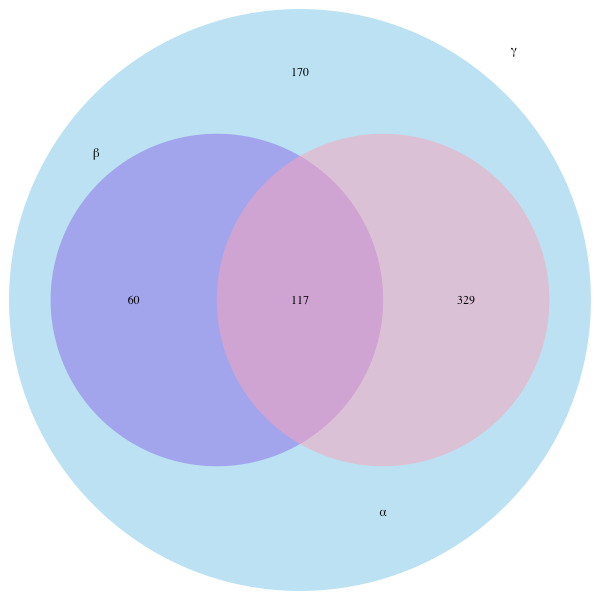
\includegraphics[width=10cm]{figures/graphs/ven_run2.png}
    \caption{Venn diagram of channel sets during interval two}
    \label{fig:venn_run2}
\end{figure}

\section{LN size}

We mentioned in \cref{subsec:information_ln} how using the fact that on-chain LN transactions used for channel creation has to be of the P2WSH type, to determine the maximum possible size of the LN. We have counted all unspent P2WSH outputs for each blockheight, in both the mainnet and the testnet. Our results is shown in \cref{fig:ln_size}, where we can see a distinct difference in the two networks: the mainnet has a more organic growth as a result of real world use, while the testnet graph is characterized by the testing which the network is used for. The sharp decline in unspent outputs on the mainnet at around block 505 000 can be explained by the sharp decline in fees for doing transactions at that time \cite{mempool_stats}, which incentivized users to consolidate their unspent outputs into fewer bigger ones. 

\begin{figure}[h]
    \centering
    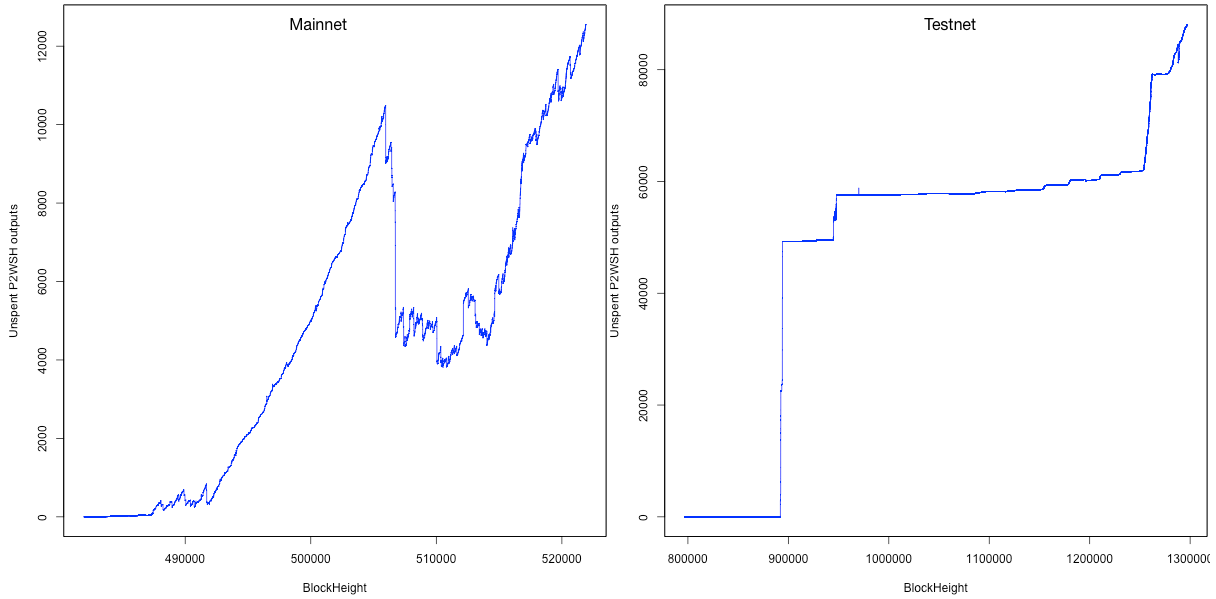
\includegraphics[width=16cm]{figures/graphs/ln_size_bc.png}
    \caption{Maximum size of the LN based on unspent P2WSH outputs on the blockchain}
    \label{fig:ln_size}
\end{figure}

While the unspent output count provides a concrete upper limit on the number of channels and therefore size of the LN, also wanted to know to which degree the amount of unspent P2WSH transactions was correlated to the size of the LN. It is clear that changes in the size of the LN will impact the number of P2WSH outputs/inputs, but there might be many other transactions not related to the LN having a larger impact. From the data we collected from the LN itself we constructed a channel count for each blockheight in the collection interval. Similarly we extracted the same block interval with the P2WSH output count from the blockchain. These two variables allowed us to compare the changes of number of channels in the LN and number of unspent P2WSH outputs. We used Kendall rank correlation coefficient \todo{check} on this data for the mainnet, which gave us a correlation coefficient of 0.73 indicating a strong positive correlation. The scatterplot for this can be seen in \cref{fig:correlation}.
We did the same for the testnet data which resulted in a coeficient of 0.45 which is only a moderate correlation. Both tests had the same p value: p < 2.2e-16.

\begin{figure}[ht]
    \centering
    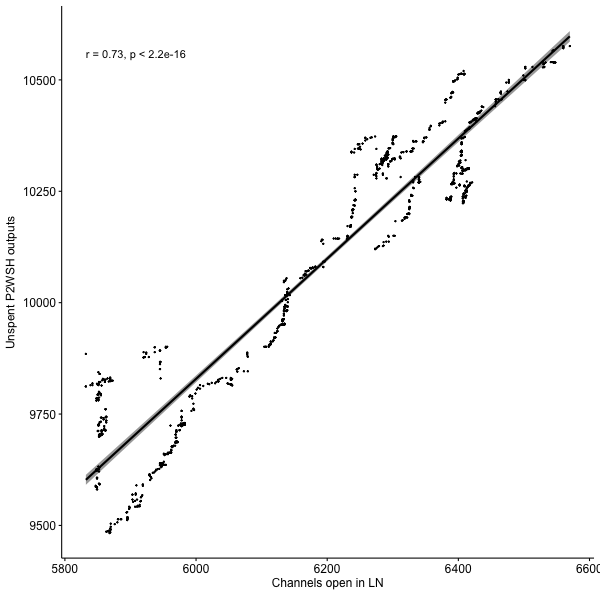
\includegraphics[width=8cm]{figures/graphs/channel_p2wsh_correlation_mainnnet.png}
    \caption{Correlation between unspent P2WSH outputs and channels open in the LN}
    \label{fig:correlation}
\end{figure}

\begin{figure}[ht]
    \centering
    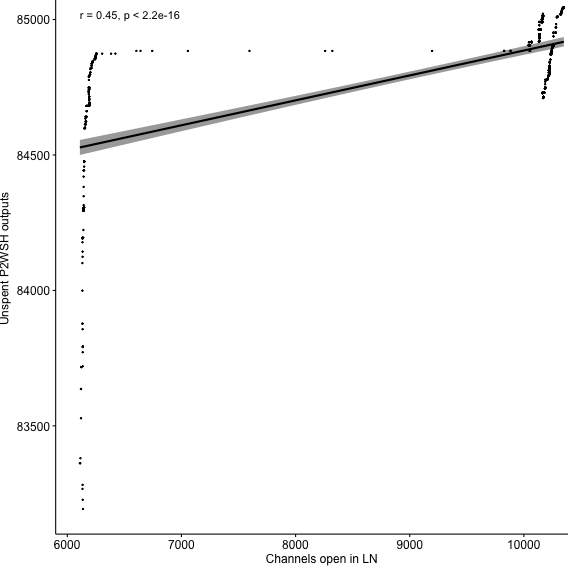
\includegraphics[width=8cm]{figures/graphs/channel_p2wsh_correlation_testnet.png}
    \caption{Correlation between unspent P2WSH outputs and channels open in the LN}
    \label{fig:correlation_testnet}
\end{figure}


\section{Channel Stats}

Using our software and the timelocked redeem scripts method for identifying channels we have parsed the blockchain on both mainnet and the testnet to the point before any P2WSH transactions and therefore channels. The result of this is data about every unilaterally closed channel that has existed. Statistics about the channels we identified can be found in \cref{subgraph_stats}. This include the number of channels fund and stats about their value and lifetime. The value of the channels is given in satoshis, with 100,000,000 satoshis being one Bitcoin. The One clear difference between the mainnet and testnet is the value used for each channel, as we briefly mentioned before coins on the testnet has no value to people, so it would be natural that they are more liberal when creating channels. 
\\

\begin{table}[ht]
\centering
\caption{Value and lifetime for channels}
\label{subgraph_stats}
\begin{tabular}{|l|c|c|c|c|}
\hline
                                             & \textbf{Mainnet} & \textbf{LN Mainnet}& \textbf{Testnet} & \textbf{LN testnet} \\ \hline
\textbf{Sample size (channels)}              & 3877             & 715           & 7 755               & 251            \\ \hline
\textbf{Average Channel value}               & 434 056          & 233 750         & 7 000 458            &7 758 942       \\ \hline
\textbf{Median channel value}                & 100 000          & 50 000         & 5 000 000            & 6 000 000        \\ \hline
\textbf{Standard Deviation Channel value}    & 1 372 703        & 586 706       & 7 096 572            & 7 191 958        \\ \hline
\textbf{Average channel lifetime}            & 1 574            & 1 940           & 2 282                & 1 269            \\ \hline
\textbf{Median channel lifetime}             & 654              & 1 836             & 396                  & 312              \\ \hline
\textbf{Standard Deviation channel lifetime} & 2 173            & 1 791           & 5 545                & 4 059            \\ \hline
\end{tabular}
\end{table}

In \cref{channel_input_output} we see the distribution for the number of inputs and outputs to channels. These results are fairy similar for both networks, we should however note the percent of channels having two outputs in relation to the percent having only one input. For the mainnet the percent of channels having one input is 70\%, and the percent of channels only having one output is 71\%. As discussed in \cref{sec:bc_analysis} we cannot easily match input - output pairs to users in the channel, so these number either means that many channels does no off-chain transactions so the single input will be outputted back to owner, or all founds in the channel ends up at one of the entities. In the testnet column we can see how the single output percentage is lower compared to the single input percent, also the double output percent is higher than the double input. This indicates that many single founded channels ends up with splitting the value when they close, and as we stated in \cref{sec:bc_analysis} this enables us to say that off-chain transactions has taken place inside the channel.
This difference is also present when we checked how many channels had the same number of inputs as outputs. On the mainnet 60\% of channels found have the same number of inputs as outputs, while on the testnet this is 49\%. 
\\

\begin{table}[]
\centering
\caption{Percentages of input - output count for channels}
\label{channel_input_output}
\begin{tabular}{|l|c|c|}
\hline
                                                                     & \textbf{Mainnet} & \textbf{Testnet} \\ \hline
\textbf{Channels with one input}             & 70.65            & 77.03            \\ \hline
\textbf{Channels with two inputs}            & 22.50            & 16.40            \\ \hline
\textbf{Channels with three inputs}          & 4.29             & 3.66             \\ \hline
\textbf{Channels with more than three inputs} & 2.56             & 2.91             \\ \hline
\textbf{Channels with one output}             & 71.74            & 52.79            \\ \hline
\textbf{Channels with two outputs}             & 27.47            & 44.52            \\ \hline
\textbf{Channels with three outputs}          & 0.65             & 1.92             \\ \hline
\textbf{Channels with more than three outputs} & 0.15             & 0.77             \\ \hline
\end{tabular}
\end{table}

\section{Linking}

We also implemented the linking methods using the heuristics described in \cref{sec:linking}, allowing us to test their effectiveness.
The linking was done, both on the set of channel graphs found during the LN collection intervals, and the total set of channels found when parsing the blockchain. In \cref{key_reuse_table} we can see the findings with regards to key reuse, when checking the entire set of channels on testnet and mainnet. Using the 3 778 channels we found on the mainnet, we extracted a total of 26270 unique keys, with 1471 or 5.5\% of these found multiple times. These keys combined where reused 3 062 times, which if the key reuse was evenly distributed in regards to the channel graphs, each channel graph would have 0.8 keys used in another channel graph. We have similar results for the testnet, where 7.2 of the keys found where reused, and 0.9 reused keys per channel graph. As discussed in \cref{sec:linking} regarding key reuse: key reuse within the same channel graph does not let us allow to link channels, but our results below does not take this into account, as we will address it later in this section.

\begin{table}[ht]
\centering
\caption{Key reuse in channel graphs}
\label{key_reuse_table}
\begin{tabular}{|l|c|c|}
\hline
                                                   & \textbf{Mainnet} & \textbf{Testnet} \\ \hline
\textbf{Unique Keys found}                         & 26989              & 47182            \\ \hline
\textbf{Unique keys reused}                        & 1511               & 3407             \\ \hline
\textbf{Instances of key reuse}                    & 3144             & 7565             \\ \hline
\textbf{Maximum number of reuses for a single key} & 23               & 171              \\ \hline
\textbf{Average reuse of keys}                     & 2              & 2.2              \\ \hline
\end{tabular}
\end{table}

We also used the two other heuristics on the channel sets, finding how many channels we where able to link using these. The results of this is shown in \cref{table:connections}. For heuristic one, where we found directly connected graphs trough outputs - inputs, we have separate results for each possible output which can be the source of such a link. We discovered a clear difference between the different outputs: the outputs from the founding transactions provide 50\% on the testnet, and 60\% percent on the mainent, of all found connections using heuristic one, compared to 2.1\% or less for the outputs from the closing transactions. The outputs from the timelocked transactions have 30\% and 33\% on the mainent and testnet respectively. One possible explanation for this difference has to do with the value of the outputs: closing and timelocked outputs are one parties value from the channel, meaning the value of these outputs is limited to the channel balance of participant owning them; outputs from the founding transaction on the other hand, is used to transfer change resulting from the output spent to found the channel, which has no size limit, meaning a output many times the value of the channel can be used. Unless using multiple inputs to found a channel, using a output from closing or timelocked transaction to create a new channel, will limit the value of the founding input to the balance in the previous channel. A possible reason for the difference between closing and timelocked outputs could be the recommendation to spend timelocked outputs discussed in \cref{sec:linking}, which if closing many channels unilatirally at one time, makes consolidation of all timelocked outputs into one timelocked transaction a natural thing to do; this would cause graph overlap, but also create a high value output from the timelocked transaction which could be used to found new channels. Heuristic 3 which used graph overlap or mutli-input timelocked transactions provided 12\% on mainnet, and 24\% on the testnet total connections found using both heuristic two and three.

\begin{table}[ht]
\centering
\caption{Relations found between channel graphs}
\label{table:connections}
\begin{tabular}{|l|c|c|}
\hline
                                       & \textbf{Mainnet} & \textbf{Testnet} \\ \hline
\textbf{Total relations found}       & 1670            & 5628             \\ \hline
\textbf{Founding output relations}   & 996               & 2828             \\ \hline
\textbf{Closing output relations}    & 30              & 2                \\ \hline
\textbf{Timelocked output realtions} & 444               & 1439             \\ \hline
\textbf{Graph overlap relations}     & 200               & 1359             \\ \hline
\end{tabular}
\end{table}

If we combine our results on the channel sets using all three heursitcs, we get a total of 4682 relations between the channel graphs in the mainnet. This enabled us to crate 4426 links between channels, becasue 71 of the relations where self relations resulting from key reuse within the same graph, and 185 redundant relationships-i.e., more than one relationship between the same channel graph with different heuristics. The set of linked channels can be seen visualized in \cref{fig:cg_mainnet_full}, where we have created a channel network as discussed in \cref{sec:linking}. The network consists of 2268 smaller components, with each node having a average degree of 2.2. While as mentioned this graph does not distinguish users, we can based on how these components is structured reveal additional information about the users participating in the channels. 
As edges represent at least one common user being present both nodes, we can create the property: for adjacent nodes there can be at most three different users, and at least two users participating. This means if the distance between vertices is more than one, we can no longer be sure of common user participation, but we cannot rule it out either. More importantly, it has a impact on a complete components-i.e., every node is connected to every other node. Because the property must hold for every node in such a complete component, there are only two possibilities with regard to user participation: there can be at most three total users in the component, or that one users participates in all nodes, but with a different second user in each, resulting in number of nodes plus one total users.
We can see a few examples of such components in \cref{fig:cg_mainnet_full}, and some components having a similar structure, but also having some additional nodes which is not part of this highly connected core.
\\

\begin{figure}[ht]
    \centering
    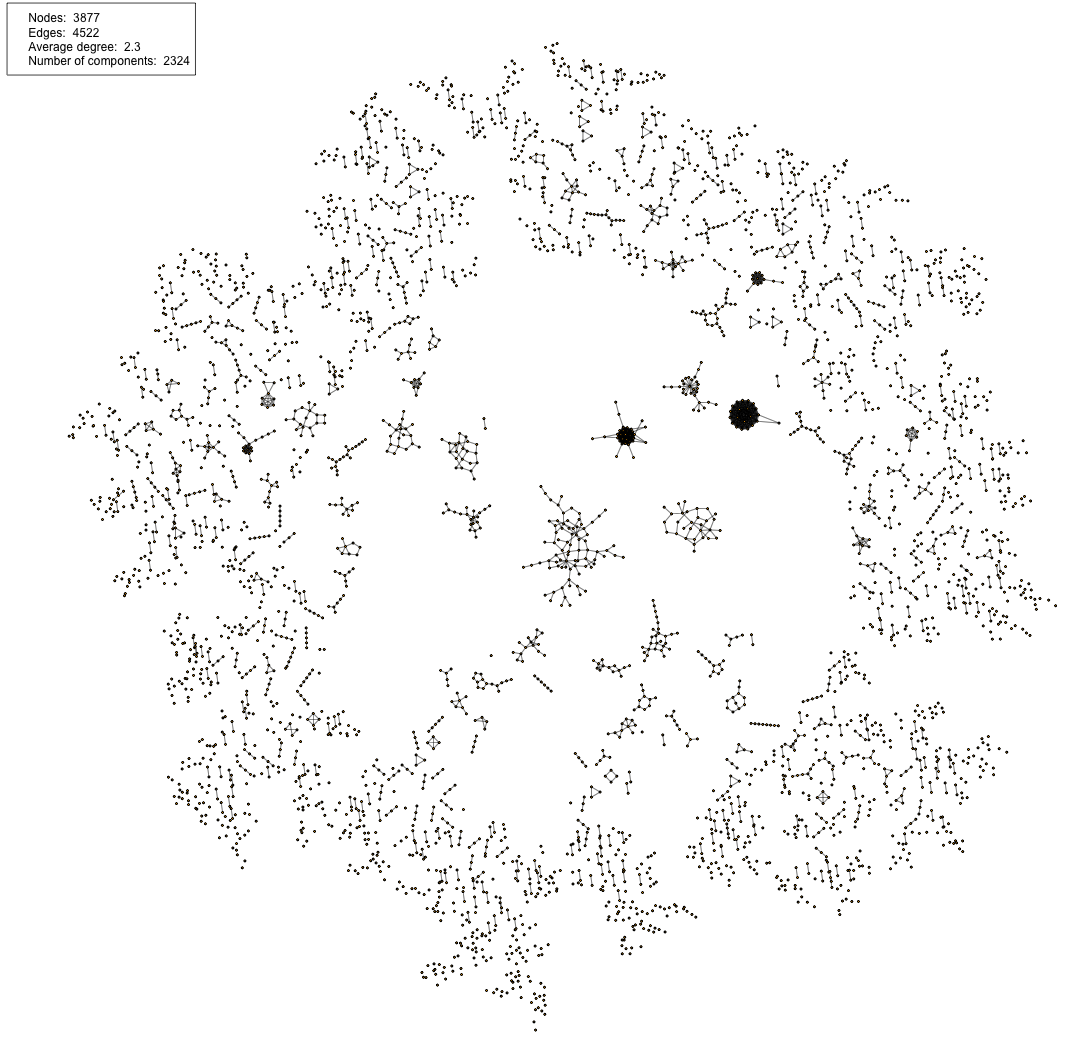
\includegraphics[width=14cm]{figures/graphs/cg_bc_mainnet_full.png}
    \caption{Channel network for mainnet}
    \label{fig:cg_mainnet_full}
\end{figure}

We also did the same as discussed in the previous paragraph for the testnet, resulting in blabllablalblabb.
The channel network shown in \cref{fig:cg_testnet_full} is more connected than the mainnet in \cref{fig:cg_mainnet_full}, with the testnet network having over twice as many nodes, but both having between 2 000 and 3 000 components. We can see this difference clearly with the large component in the middle of the testnet graph. As the LN is one network, it should consist of one dynamic component, so a historic network graph should also ideally have one large component. While we can see this beginning to emerge in our testnet channel network, it is very clear in the channel network constructed using LN data as seen in \cref{fig:channel_network_LN_mainent}.
\\

\begin{figure}[ht]
    \centering
    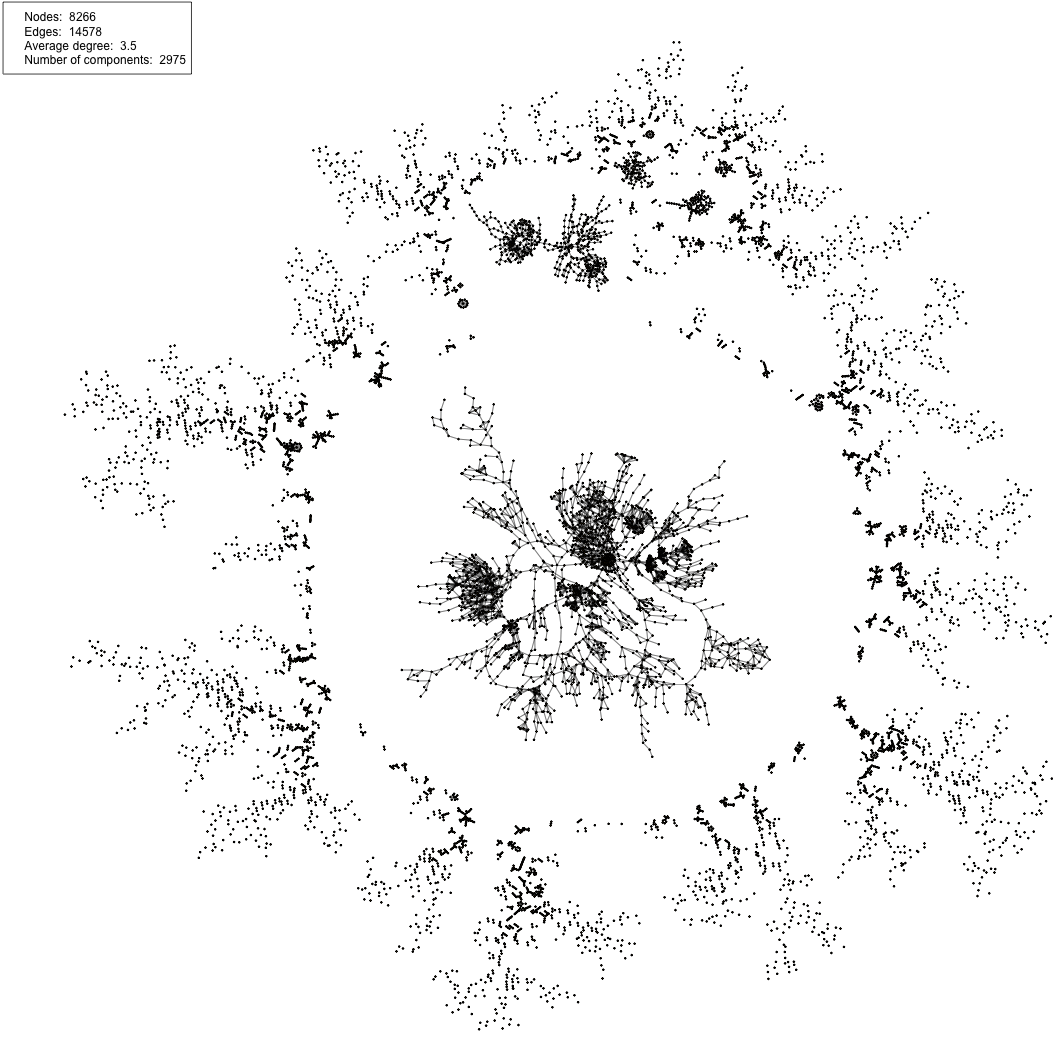
\includegraphics[width=14cm]{figures/graphs/cg_bc_testnet_full.png}
    \caption{Channel network for testnet}
    \label{fig:cg_testnet_full}
\end{figure}

The channel network in \cref{fig:channel_network_LN_mainent} based on LN data, was created for comparing with the networks we crated based on linking blockchain information. In the LN data we collected in the intervals we used the node id, which identifies a node/user, to link the channels that node participated in. While users are easily separable by this id, we ignored this to create the same type of network as we did using the blockchain data, meaning edges only indicate common user participation, not a specified user. 
As shown in \cref{fig:channel_network_LN_mainent} the network is highy connected with the 715 nodes having a average degree of 115. We can see that almost all nodes part of the main component, with some nodes in the center having a very high degree.
If we compare this to the channel network in \cref{fig:channel_network_BC_mainnet}, which we cratered using the channels identified on the blockchain in the same interval, and linked using our three intervals, we can see how limited our linking capabilities are.


\begin{figure}[ht]
    \centering
    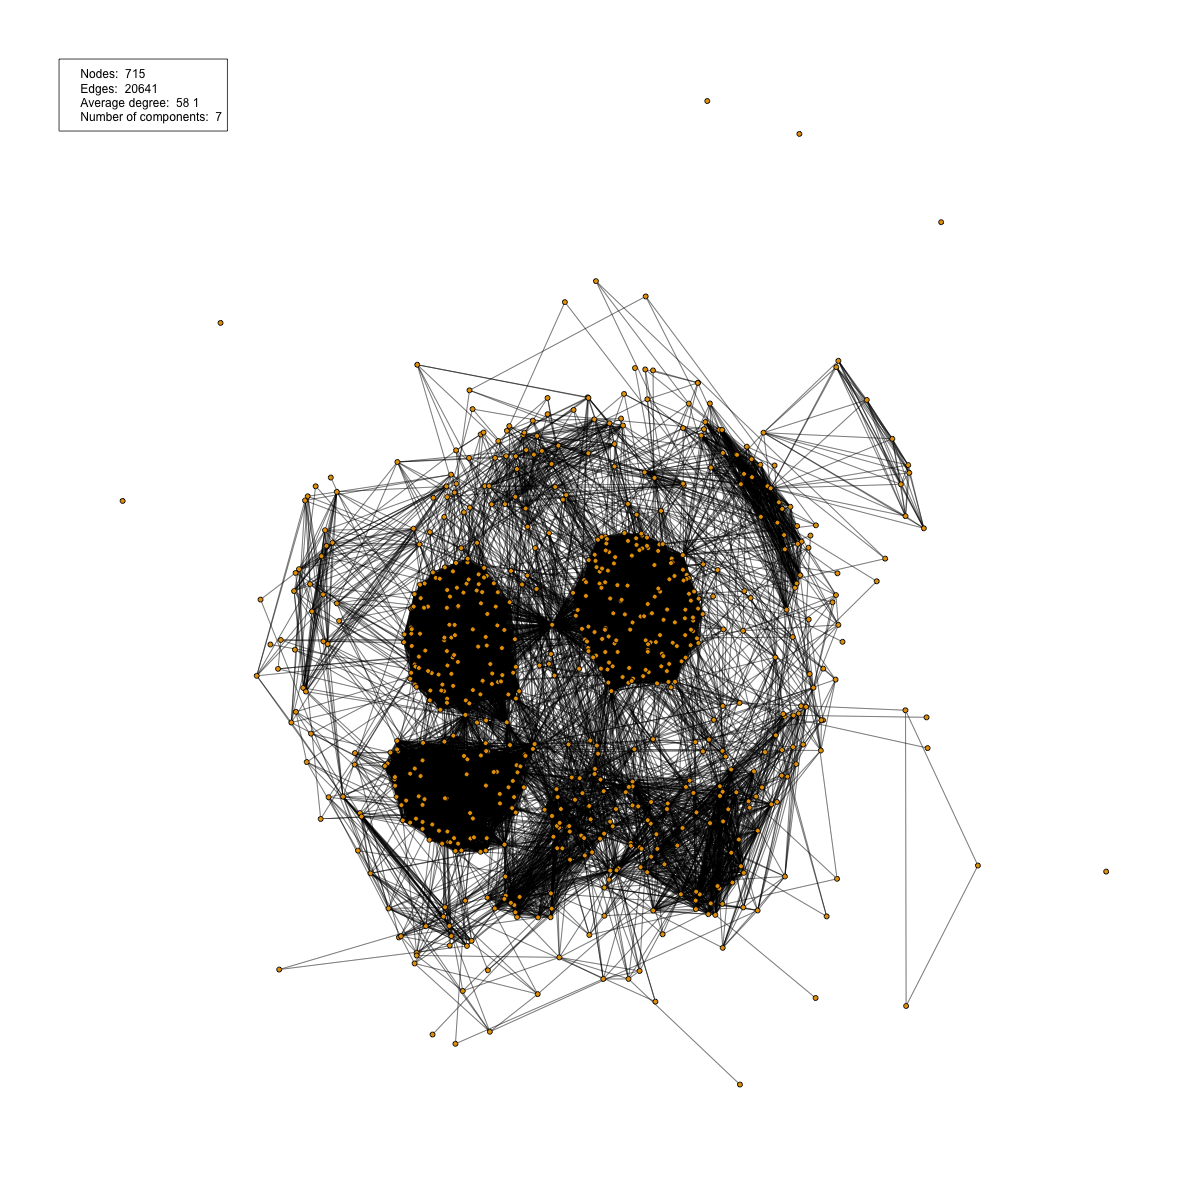
\includegraphics[width=13cm]{figures/graphs/cg_ln_mainnet_run1.png}
    \caption{Linked channels from the LN, mainnet, first interval}
    \label{fig:channel_network_LN_mainent}
\end{figure}

\begin{figure}[ht]
    \centering
    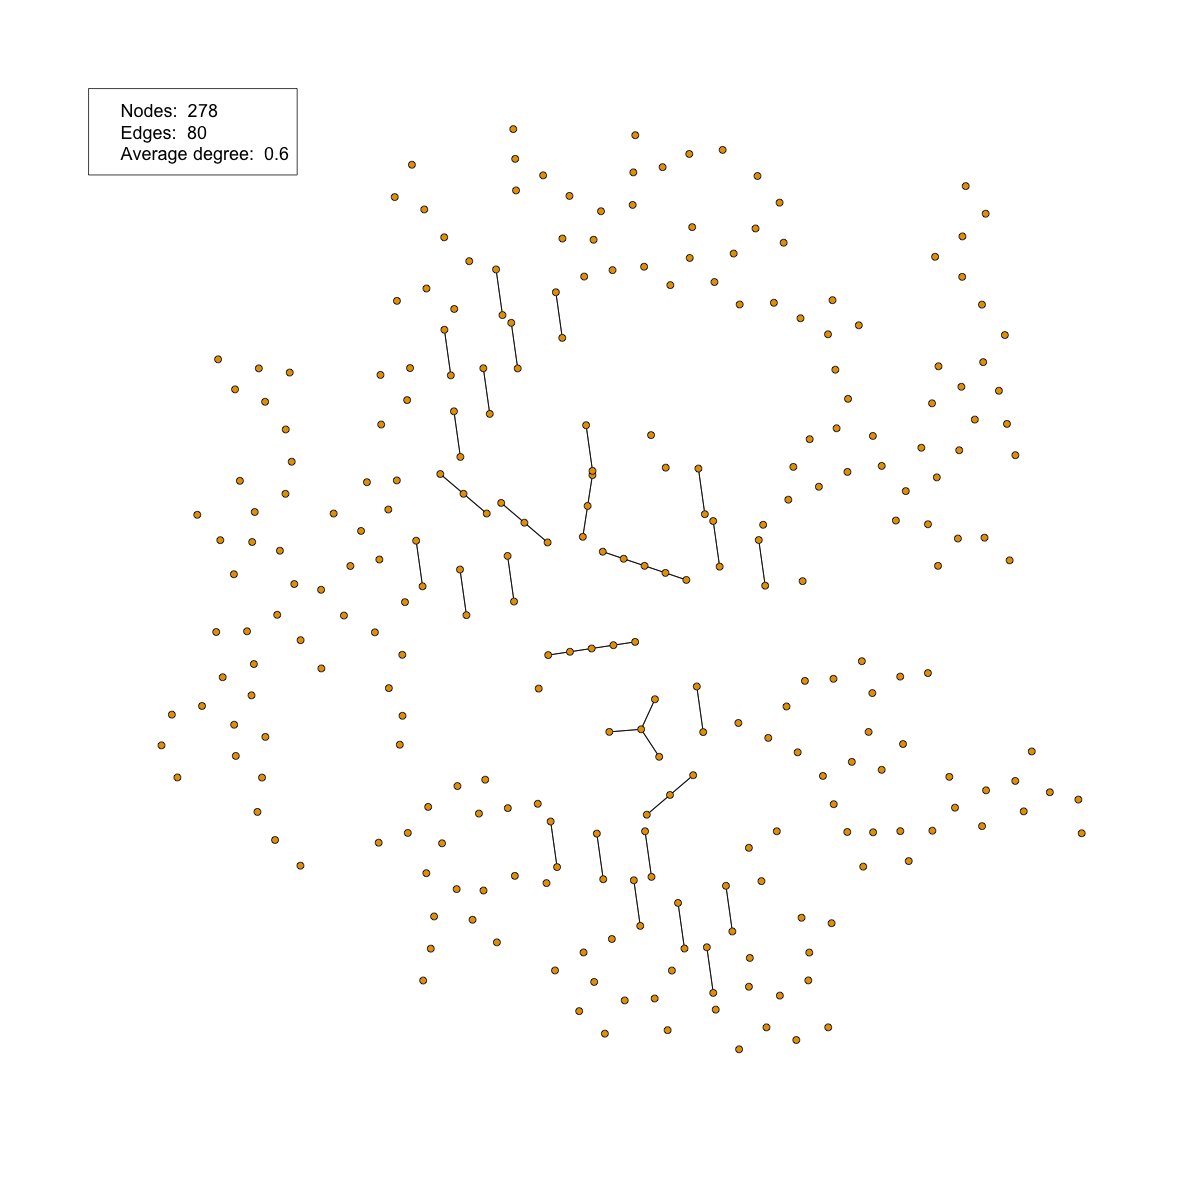
\includegraphics[width=13cm]{figures/graphs/cg_bc_mainnet_run1.png}
    \caption{Linked channels from the blockchain, mainnet, first interval}
    \label{fig:channel_network_BC_mainnet}
\end{figure}